\documentclass{article}
\usepackage[utf8]{inputenc}

\usepackage{tikz}
\usetikzlibrary{positioning}



\title{Kafka Project}
\author{Mislav Jakšić}
\date{\today{}}



\begin{document}

\maketitle

Use Java 8

Use Spring Boot to implement a REST API

Assume an intranet for the purpose of security

Hamag Bicro agency, a big project

Construct a minimal UI for testing

Construct the project CRUDL stripe by CRUDL stripe (create, read, update, delete, list)

Use zkClient to connect to Zookeeper

Use AdminClient to connect to Kafka

Use Kafka version 2.1 or 0.11

Consider multiple architectures: microservices, monolith ili client server

It is impossible to create all CRUDL operations for each resource

The important Kafka resources are: topics, partitions, messages, consumers, producers, streams

Wrap each and every Kafka functions in your own function to prevent API changes from effecting the project

Make notes about naming conventions

Take notes about Kafka resources and API

Always have the bigger picture in mind

Monitoring sems to be a bitmore important then CRUDL operations

Take notes about the different preexisting solutions and libraries

Abstract the configuration



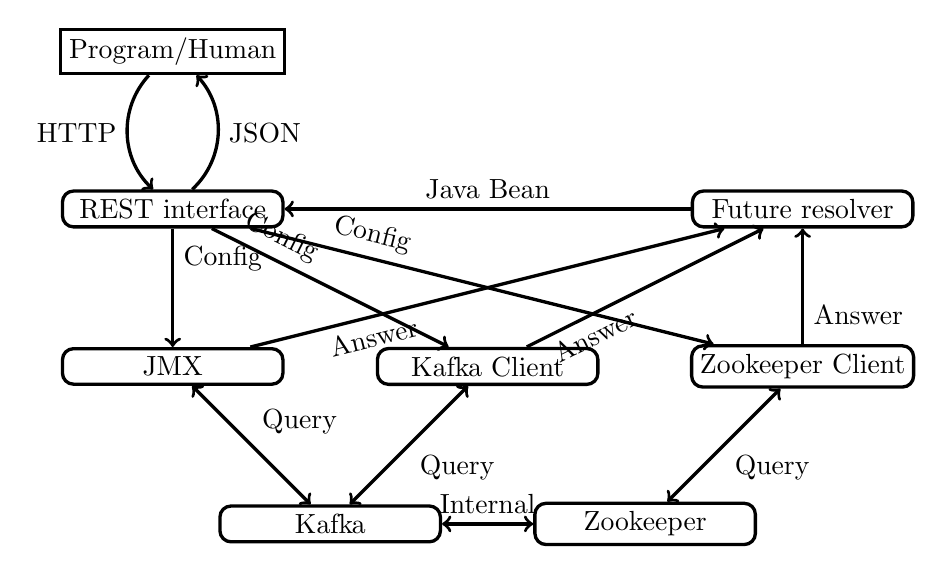
\begin{tikzpicture}[ % has a lot of options; consult the pgf manual
bend angle=45,
square/.style={rectangle, draw=black, fill=white, very thick, inner sep=3pt, minimum width=28mm},
rounded_square/.style={rectangle, rounded corners, draw=black, fill=white, very thick, inner sep=3pt, minimum width=28mm},
both_arrow/.style={<->, very thick},
out_arrow/.style={->, very thick},
in_arrow/.style={<-, very thick},
above_edge_text/.style={above, midway, sloped}
]

% \node[type](name_of_node)[above/below/right/left/...=of name_of_node]{node_text}
%   edge[<->, bend left/right] node[auto, swap]{edge_text}(out_name_of_node)
% OR
% \node[type](name_of_node)[above/below/right/left/...=of name_of_node]{node_text}
\node[square](users) at (0,0) {Program/Human};

\node[rounded_square](REST_interface) at (0,-2) {REST interface};
\node[rounded_square](future_resolver) at (8,-2) {Future resolver};

\node[rounded_square](jmx) at (0,-4) {JMX};
\node[rounded_square](kafka_client) at (4,-4) {Kafka Client};
\node[rounded_square](zookeeper_client) at (8,-4) {Zookeeper Client};

\node[rounded_square](kafka) at (2,-6) {Kafka};
\node[rounded_square](zookeeper) at (6,-6) {Zookeeper};

% \draw[->](name_of_node.direction) -- (name_of_node.direction)
% OR
% \draw[->](name_of_node.direction) to [bend right] node[]{edge_text} (name_of_node.direction)
% OR
% \draw[->](name_of_node.direction) .. controls +(up/down/right/left:10mm) and +(up/down/right/left:10mm) .. (name_of_node.direction);
\draw[out_arrow](users) to [bend right] node[auto,swap]{HTTP} (REST_interface);
\draw[out_arrow](REST_interface) to [bend right] node[auto,swap]{JSON} (users);

\draw[out_arrow](REST_interface) to [] node[auto,near start]{Config} (jmx);
\draw[out_arrow](REST_interface) to [] node[auto,near start,sloped]{Config} (kafka_client);
\draw[out_arrow](REST_interface) to [] node[auto,near start,sloped]{Config} (zookeeper_client);

\draw[out_arrow](future_resolver) to [] node[auto,swap]{Java Bean} (REST_interface);

\draw[out_arrow](jmx) to [] node[auto,swap,near start,sloped]{Answer} (future_resolver);
\draw[out_arrow](kafka_client) to [] node[auto,swap,near start,sloped]{Answer} (future_resolver);
\draw[out_arrow](zookeeper_client) to [] node[auto,swap,near start]{Answer} (future_resolver);

\draw[both_arrow](jmx) to [] node[auto]{Query} (kafka);
\draw[both_arrow](kafka_client) to [] node[auto]{Query} (kafka);
\draw[both_arrow](zookeeper_client) to [] node[auto]{Query} (zookeeper);

\draw[both_arrow](kafka) to [] node[auto]{Internal} (zookeeper);

\end{tikzpicture}

\end{document}
